\begin{tikzpicture}[
    grow=right,
    level 1/.style={sibling distance=3.5cm,level distance=5.2cm},
    level 2/.style={sibling distance=3.5cm, level distance=6.7cm},
    edge from parent/.style={very thick,draw=blue!40!black!60,
        shorten >=5pt, shorten <=5pt},
    edge from parent path={(\tikzparentnode.east) -- (\tikzchildnode.west)},
    kant/.style={text width=2cm, text centered, sloped},
    every node/.style={text ragged, inner sep=2mm},
    punkt/.style={rectangle, rounded corners, shade, top color=white,
    bottom color=blue!50!black!20, draw=blue!40!black!60, very
    thick }
    ]

\node[punkt, text width=5.5em] {lego-character}
    %Lower part lv1
    child {
        node[punkt] [rectangle split, rectangle split, rectangle split parts=4,
         text ragged] {
            \textbf{character}
                  \nodepart{second}
            name
                  \nodepart{third}
            jedi?
            	  \nodepart{fourth}
            force	  
        }
        edge from parent
            node[kant, below, pos=.6] {}
    }
    %Upper part, lv1
    child {
        node[punkt, text width=6em] {Figure}
        %child 2
            edge from parent{
                node[kant, above] {}}
    };
\end{tikzpicture}\\
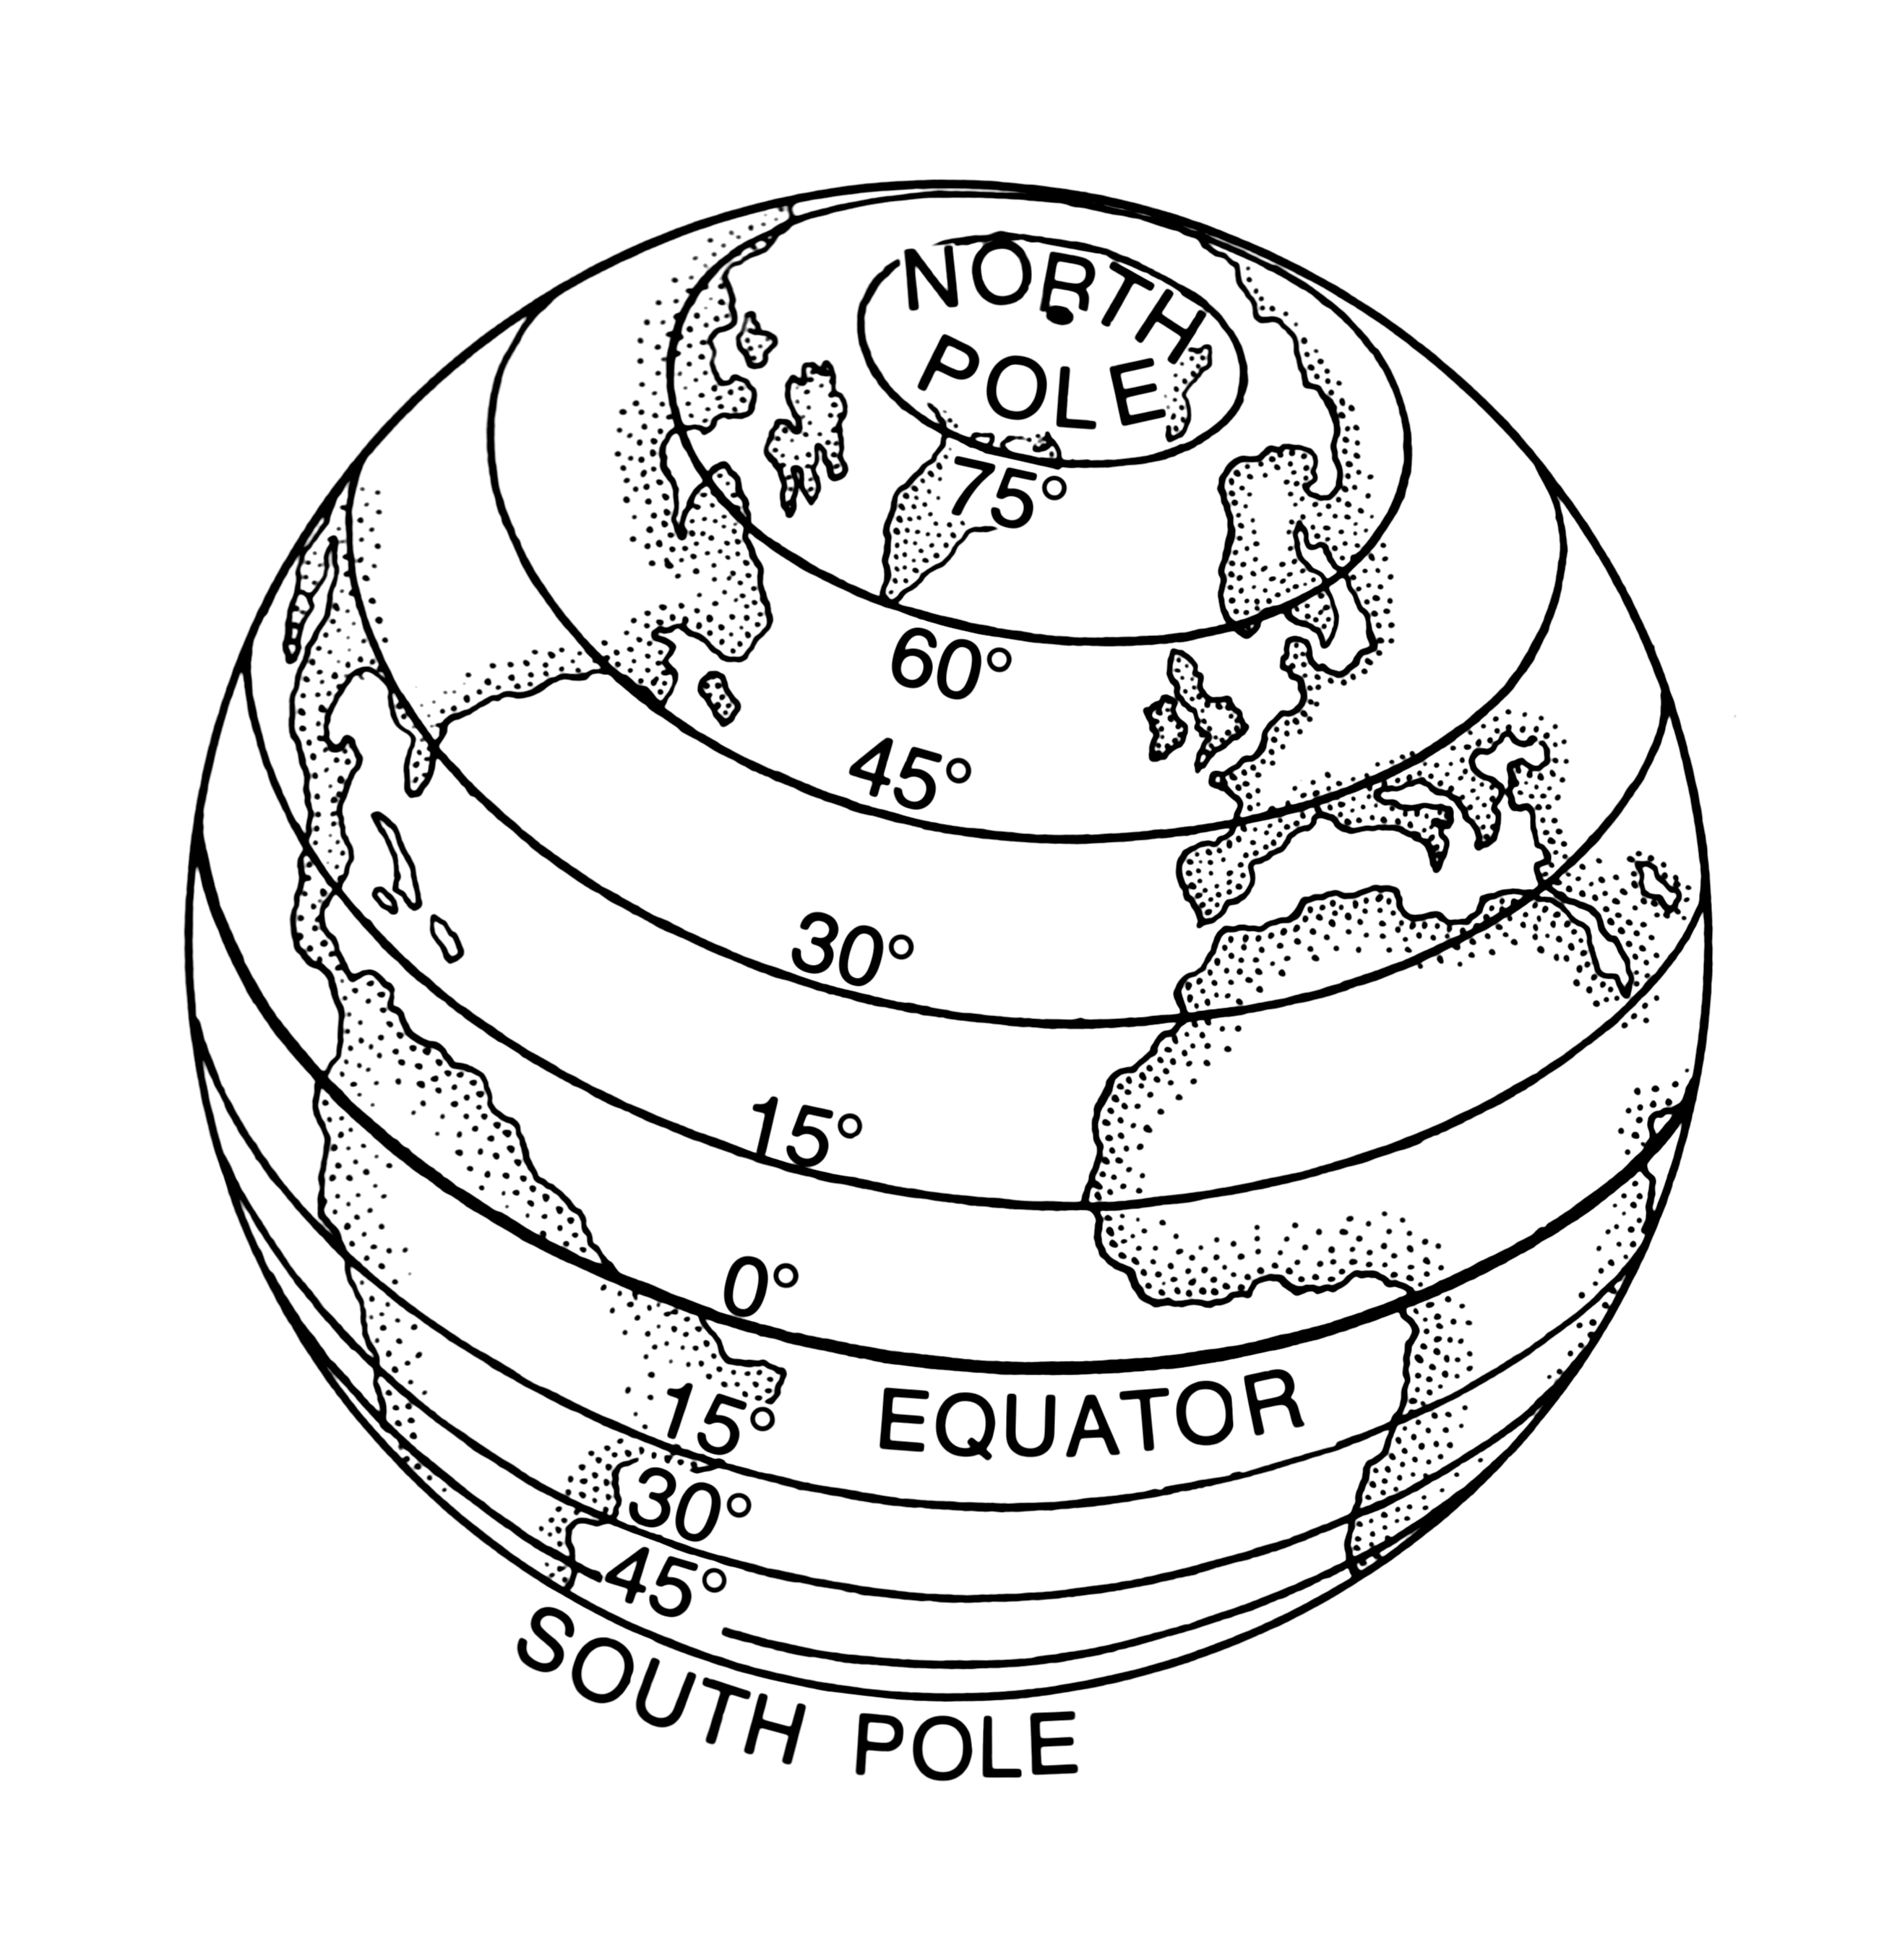
\includegraphics[scale=0.5]{Latitude}
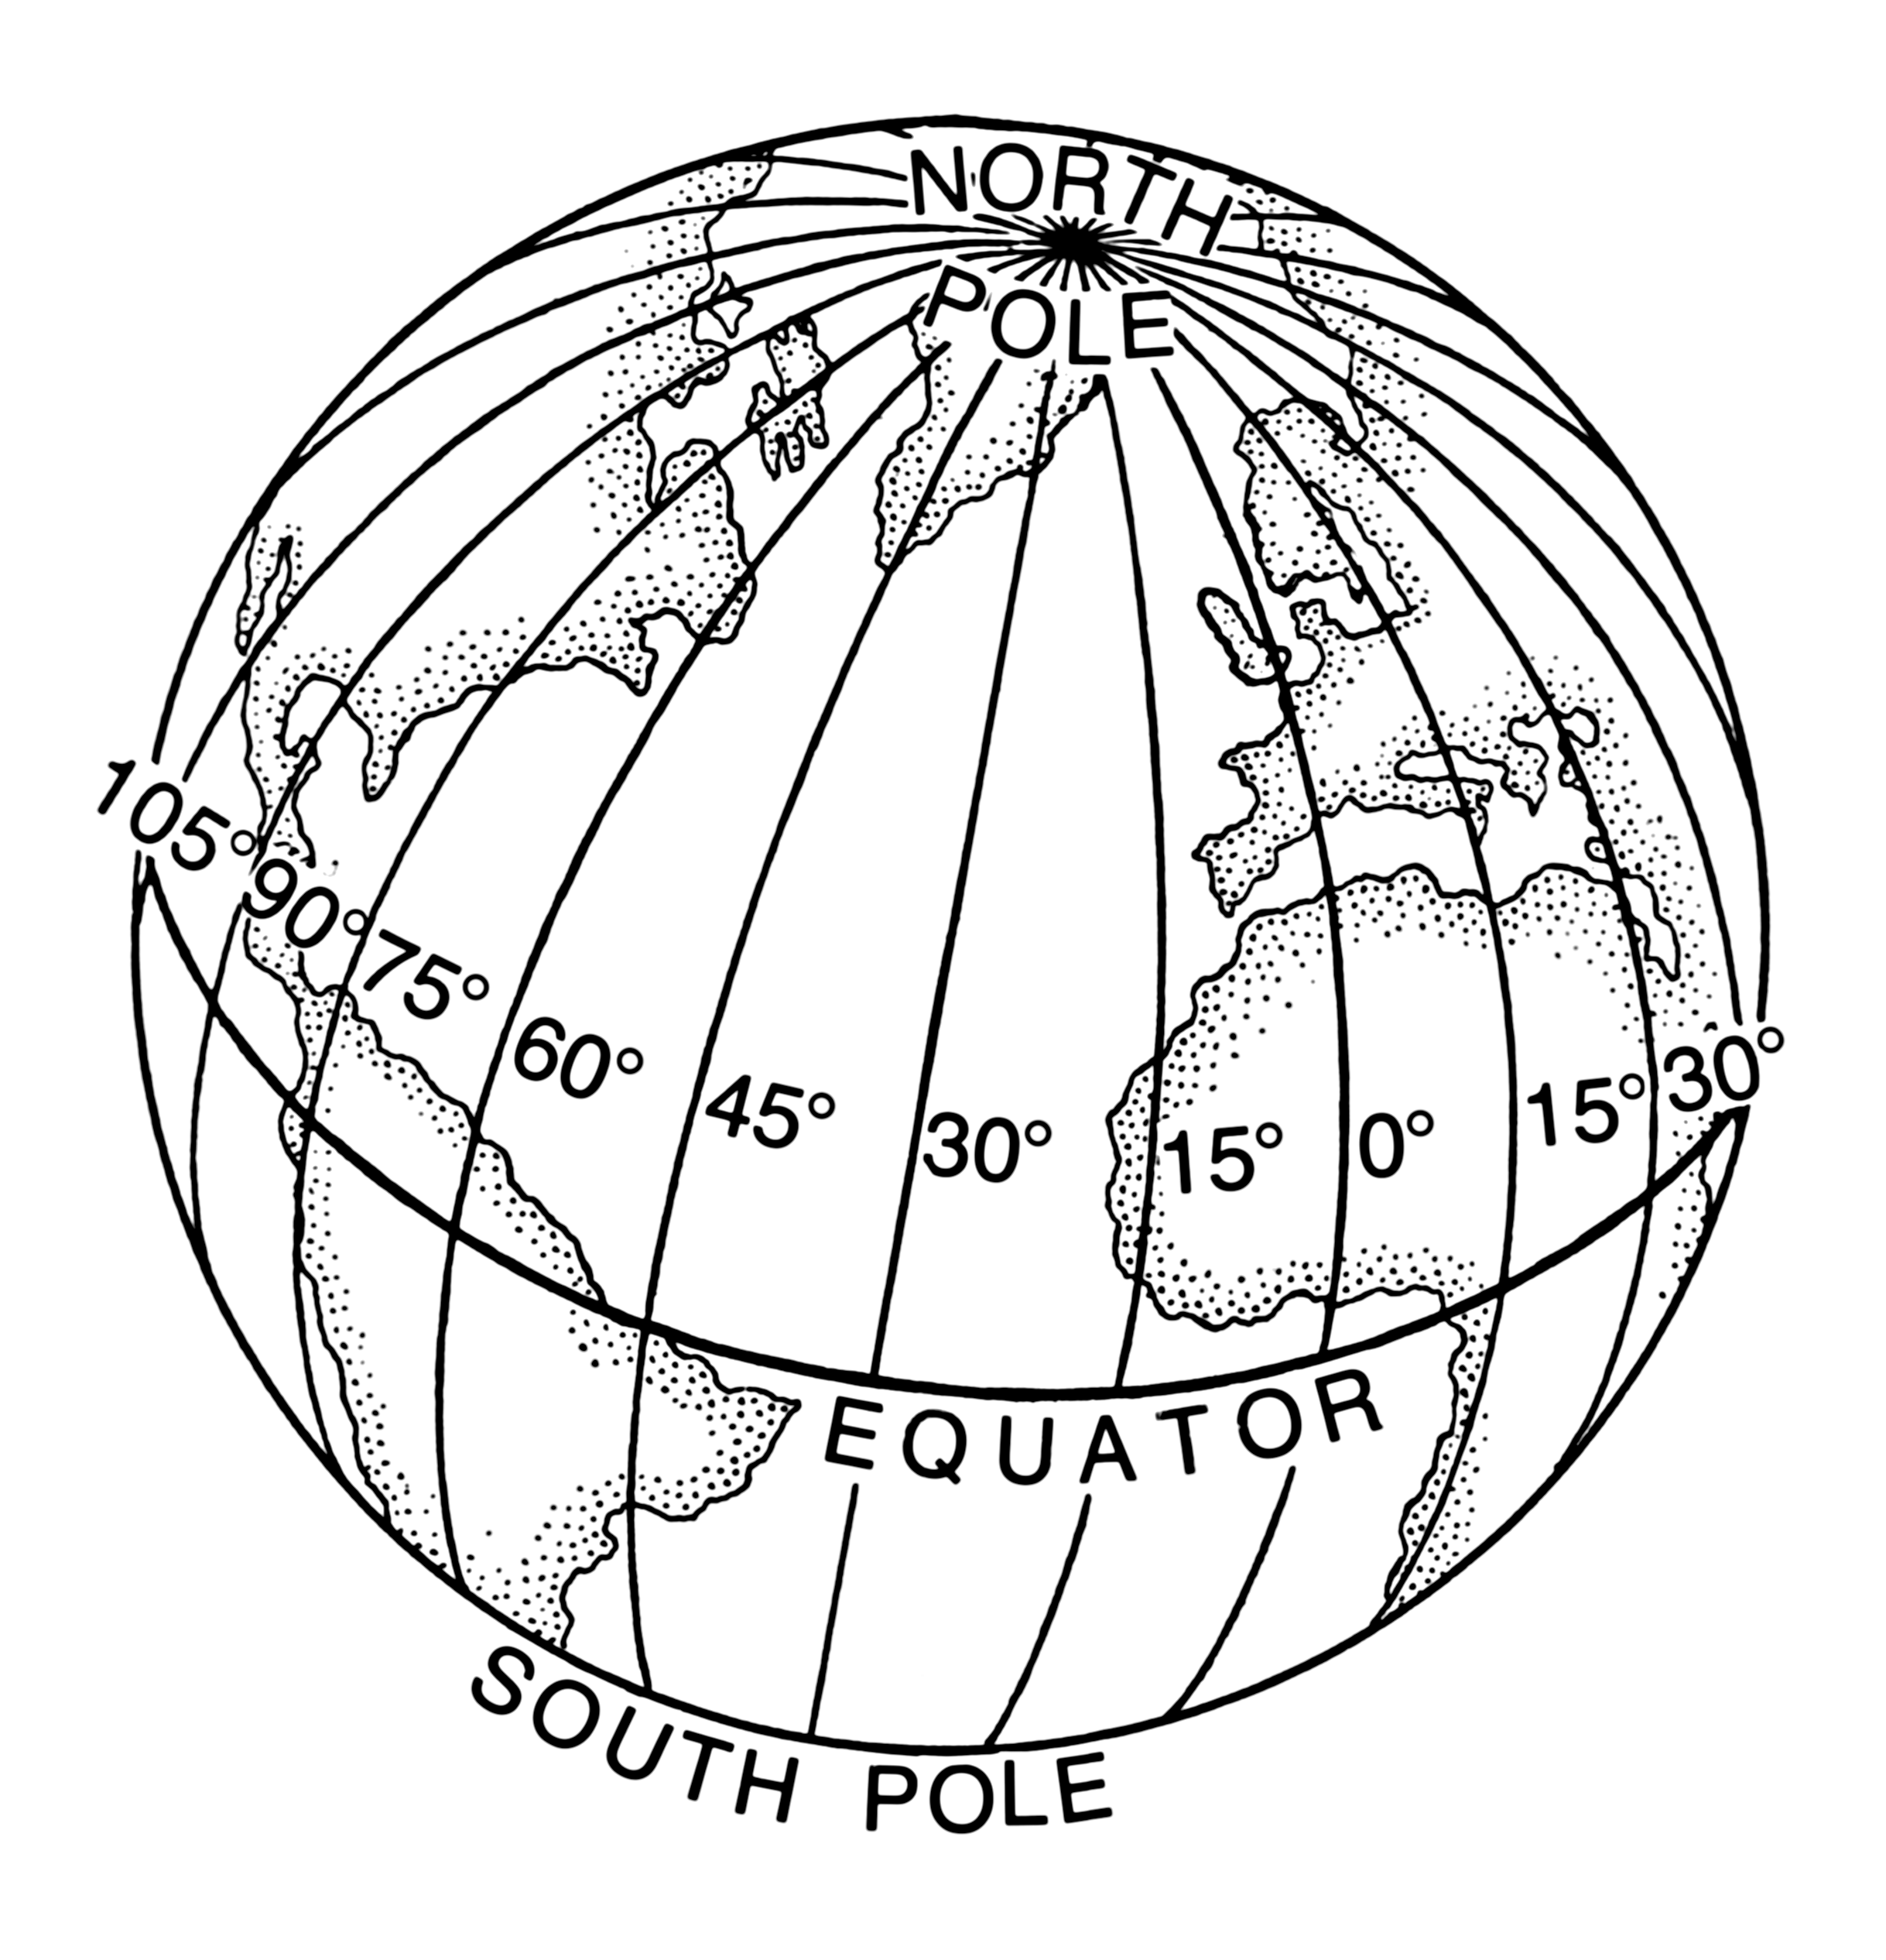
\includegraphics[scale=0.5]{Longitude}\\
Position Nord/Südwest vom Äquator Position west/östlich vom Nullmeridian\\
Sei \auf$p$\zu ein Prädikat mit Signatur \textcolor{pseudo}{(\argt{} -\zu boolean)}.\\
Eine Signatur der Form \textcolor{pseudo}{(predicate \auf p\zu)} gilt für jeden Wert der Signatur \argt{} sofern (\auf p\zu) \eval \#t\\
Signaturen des Typs \textcolor{pseudo}{(predicate \auf p\zu)} sind damit \underline{spezifischer} (restriktiver) als die Signatur \argt{} selbst.\\
\textcolor{pseudo}{(define \auf newt\zu (signature \auf t\zu))}\\
\underline{Beispiele:}
\begin{lstlisting}
(define farbe
	(signature (one-of "Blatt" "Herz" "Blatt" "Eichel" "Schell")))
\end{lstlisting}
\begin{lstlisting}[frame = single]
; Ist x ein gültiger Breitengrad 
; zwischen Südpol (-90@\latexcode{$^{\circ}$}@) und Nordpol (90@\latexcode{$^{\circ}$}@)?
(: latitude? (real -> boolean))
(check-expect (latitude? 78) #t)
(check-expect (latitude? -92) #f)
(define latitude?
  (lambda (x)
    (within? -90 x 90)))


; Ist x ein gültiger Längengrad westlich (bis -180@\latexcode{$^{\circ}$}@) 
; bzw. östlich (bis 180@\latexcode{$^{\circ}$}@) des Meridians?
(: longitude? (real -> boolean))
(check-expect (longitude? 0) #t)
(check-expect (longitude? 200) #f)
(define longitude?
  (lambda (x)
    (within? -180 x 180)))


; Signaturen für Breiten-/Längengrade basierend auf
; den obigen Prädikaten
(define latitude
  (signature (predicate latitude?)))
(define longitude
  (signature (predicate longitude?)))

\end{lstlisting}